
%(BEGIN_QUESTION)
% Copyright 2007, Tony R. Kuphaldt, released under the Creative Commons Attribution License (v 1.0)
% This means you may do almost anything with this work of mine, so long as you give me proper credit

Examine this liquid flow controlling system, using two flow switches and a motor-actuated control valve.  Then, answer the questions that follow:

$$\includegraphics[width=15.5cm]{i01814x01.eps}$$

$$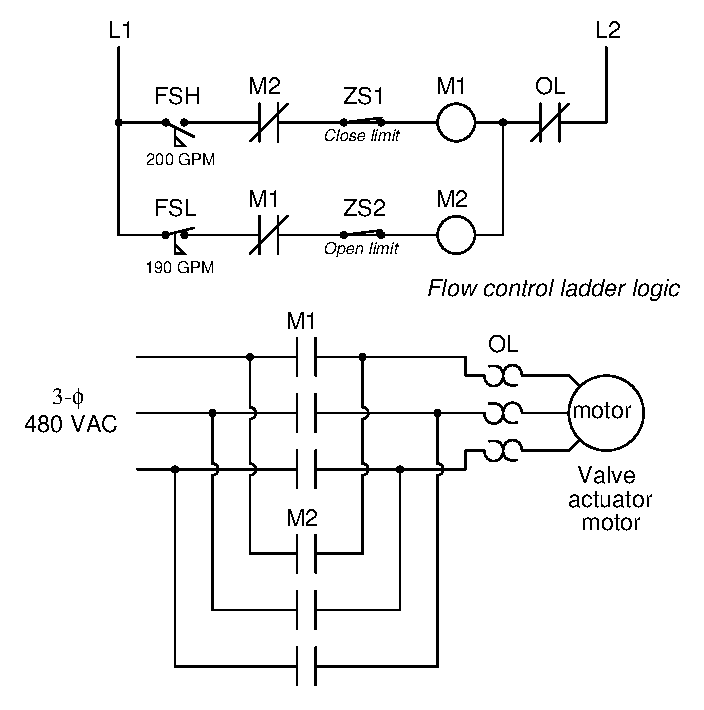
\includegraphics[width=15.5cm]{i01814x02.eps}$$

\begin{itemize}
\item{} Which motor contactor (M1 or M2) opens the valve?  Which one closes the valve?
\item{} How will the control valve respond if the flow is continually below 190 GPM?
\item{} What purpose does each normally-closed ``M'' contact serve?
\item{} Would you say this control circuit performs a {\it proportional} action or an {\it integrating} action?  Why??
\end{itemize}

\underbar{file i01814}
%(END_QUESTION)





%(BEGIN_ANSWER)

If the flow rate is continually below 190 GPM, the valve will continue to open wider and wider, until (eventually) the ``Open limit'' switch actuates and stops the motor.

%(END_ANSWER)





%(BEGIN_NOTES)

Even though the only ``sensor'' here is a pair of switches, this control circuit is integrating in nature.  It drives the valve either open or closed at a constant rate (set by motor speed) if the flow is not within the bounds set by the two switches' trip points.

$$\includegraphics[width=15.5cm]{i01814x01.eps}$$

$$\includegraphics[width=15.5cm]{i01814x03.eps}$$

\vskip 20pt \vbox{\hrule \hbox{\strut \vrule{} {\bf Virtual Troubleshooting} \vrule} \hrule}

This question is a good candidate for a ``Virtual Troubleshooting'' exercise.  Presenting the diagram to students, you first imagine in your own mind a particular fault in the system.  Then, you present one or more symptoms of that fault (something noticeable by an operator or other user of the system).  Students then propose various diagnostic tests to perform on this system to identify the nature and location of the fault, as though they were technicians trying to troubleshoot the problem.  Your job is to tell them what the result(s) would be for each of the proposed diagnostic tests, documenting those results where all the students can see.

During and after the exercise, it is good to ask students follow-up questions such as:

\begin{itemize}
\item{} What does the result of the last diagnostic test tell you about the fault?
\item{} Suppose the results of the last diagnostic test were different.  What then would that result tell you about the fault?
\item{} Is the last diagnostic test the best one we could do?
\item{} What would be the ideal order of tests, to diagnose the problem in as few steps as possible?
\end{itemize}

%INDEX% Control, integral: differential gap flow control

%(END_NOTES)


